\chapter{Implementation}\label{ch:implementation}
In this chapter I would like to present the technologies that were used while implementing the previously described system.
During the development,
base package of the application was named \inlinecode{OLB},
which is an acronym for \textbf{O}ptimization \textbf{L}oad \textbf{B}alancer.
In the following pages, 
the developed application is called this way.

The implementation itself was focused mainly on load balancing algorithm 
and on system's core.
What is not part of this paper,
and belongs to future work (described in section \ref{sec:future-work}),
is an execution module, 
which would be able to perform the decisions made by the core algorithm presented 
and implemented in this thesis.

\section{Architecture}\label{sec:architecture}

Although this paper focuses only on scheduling system's core,
the architecture keeps in mind future work on whole infrastructure.
Therefore us the system's architecture based on the idea of cooperating microservices,
where each service has control over specific part of the infrastructure. 

Microservice architecture is an software design architectural style 
that structures an application as a collection of loosely coupled services that 
are organized around system's business capabilities\cite{namiot2014micro} 
and are independently deployable with enabled continuous delivery\cite{balalaie2016microservices}.
Microservice architectural design also helps to system's better horizontal scalability
by using multiple instances of one microservice 
and orchestration module.


\subsection{Architecture scheme}\label{subsec:architecture-scheme}
Scheme \ref{fig:scheduling-core-arch} visualizes only system's core architecture. 
However,
whole design keeps in mind future infrastructure development proposed in section \ref{sec:future-work}.
Implementation itself was developed accordingly 
and used technologies and techniques are described in following sections.

\begin{figure}[ht]
    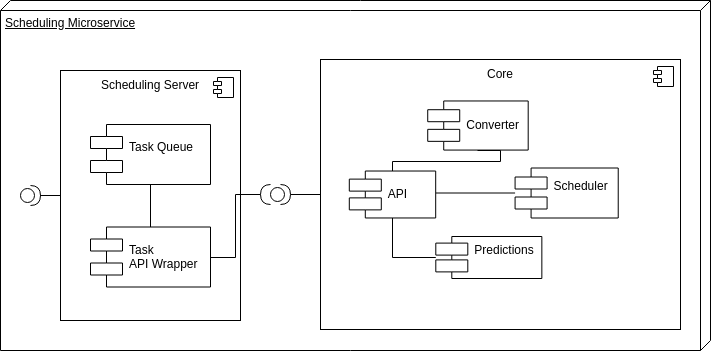
\includegraphics[width=\textwidth]{i_scheduler.png} 
    \centering
    \caption{Microservice architecture with scheduling core}
    \label{fig:scheduling-core-arch}
\end{figure}

Core component, 
which is responsible for scheduling and load balancing,
is composed of API, converter, predictions and scheduler module.
\begin{itemize}
    \item \textit{API module} implements common core interface \inlinecode{OlbCoreApi} 
    and is responsible for scheduling requests handling.
    Actual implementation of API interface is class \inlinecode{OlbCoreApiImpl}.
    \item \textit{Converter module} is used to convert received input data into inner scheduler data representation 
    and then back to common data transfer objects. 
    This converter is implemented as a class \inlinecode{InputToDomainConverter}.
    \item \textit{Scheduler module} contains constraints, evaluator and scheduling system based on OptaPlanner solution
    (described in section \ref{sec:load-balancing-optaplanner}).
    Scheduler module consist of multiple packages, 
    \inlinecode{constraints} - containing all constrains for scheduling algorithm,
    \inlinecode{domain} with defined scheduling domain for OptaPlanner,
    \inlinecode{evaluation} which includes evaluator calculating planning score
    and \inlinecode{solver} package with factory initializing OptaPlanner scheduling core.
\end{itemize}

Scheduling server provides HTTP API access to the core
and serves as microservice base.
Server module is based on Ktor framework (described in section \ref{subsec:framework})
that runs under the hood and provides HTTP functionality.

In the current implementation,
server API accepts binary serialized data transfer objects
instead of common JSON or XML.
This is because of number of interfaces and loosely coupled data objects,
that are being used in the application.
Migration to JSON technology is addressed in future work in section \ref{sec:future-work}.

\subsubsection{Simulations architecture}\label{subsec:simulations-architecture}
Simulations module (project module \inlinecode{simulations}) is designed as another microservice to simulate future load balancing system's behavior.
Following figure \ref{fig:simulations-arch} shows architecture of the module.  

\begin{figure}[ht]
    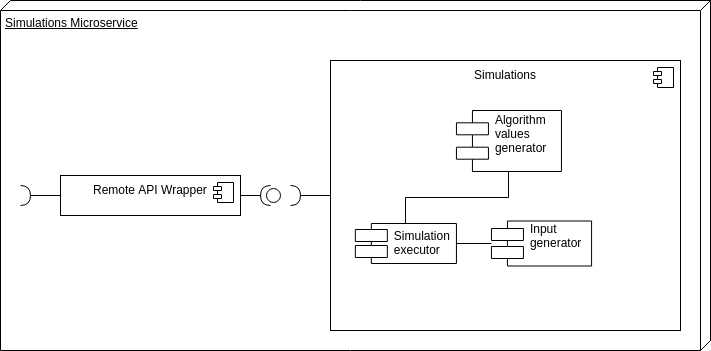
\includegraphics[width=\textwidth]{i_simulations.png}
    \centering
    \caption{Simulations module scheme}
    \label{fig:simulations-arch}
\end{figure}

Input data are generated by input generator module,
which can be found for example in \inlinecode{DomainBuilder} class.
Algorithm values are parsed from file in class \inlinecode{DataParser} 
and corresponding model is created on top of them in \inlinecode{JobWithHistoryFactory}.

Remote API wrapper is used to create connection between remote microservice, with scheduling API, and simulation.
For the simulation module,
the connection seems to be synchronous.
This is because there is a blocking queue used to store and answer the calls between these two microservices.
Thanks to this solution,
simulations can be run in microservices mode as well as locally without any additional effort needed.
Remote scheduling solution is implemented in project module \inlinecode{remote-scheduler}.
Local simulations can be found for example in \inlinecode{OnePlanningRoundMain} or \inlinecode{ExecutionConfiguration} classes.

\section{Development stack}\label{sec:development-stack}
The development stack is based on the Java platform, 
targeting primarily JVM 11\footnote{Java Virtual Machine - runtime environment for Java byte code}
but including backwards compatibility with JVM 8.
However, 
the traditional Java platform programming language Java was not used.

\subsection{Programming Language}\label{subsec:programming-language}
The OLB\footnote{Optimization Load Balancer, name of the application} is not bound to the single technology, 
which could limit the development stack and for that reason,
we had a free choice while choosing the programming language used for the OLB implementation.

OLB is programmed in the programming language \textbf{Kotlin}.
This cross-platform, statically typed, the general-purpose programming language is developed by JetBrains\cite{kotlinReference}.
Kotlin is 100\% interoperable with Java because it uses JVM as its runtime and it is compiled to the Java Bytecode.
Apart from the Java Bytecode, it can also be compiled to JavaScript or native code.\cite{kotlinReference}
The main advantage of Kotlin is its aggressive and robust type inference,
meaning that for the most of the time,
it is not necessary to specify used data type since Kotlin compiler can infer it from the context.\cite{kotlinReference}
It results in concise language syntax and therefore to the faster development in general.

Another great advantage is Kotlin's \textit{null safety}. 
Kotlin compiler distinguishes between non-nullable types and nullable types 
and enforces \textit{null checks}\footnote{Check whether the object being used has not null value} when the object has a nullable data type.
This feature effectively leads to fewer problems in the code
and drastically reduces \textit{Null Pointer Exceptions}\footnote{Exception raised when code access reference that has null value}
during the runtime.

\subsection{Build environment}
The application uses Gradle as its build automation system.
It was chosen mainly because its incrementally build system,
that works by tracking input and output of tasks, 
including files changes tracking, and only running tasks, that are necessary
and thus reducing the required time to build the project. 
Also, it processes only these files that were changed between tasks execution. 
Another reason we choose Gradle was that it is preferred build system for Kotlin.

The preferred approach to assemble the application is to use Docker
and build it as the Docker image, 
which can be then run inside the Docker container.

\subsubsection{Docker build environment}
To keep the build clean and reusable on almost every operating system and 
machine setup we decided to use 
\textbf{multistage Docker build}\footnote{Docker is a technology that performs operating-system-level virtualization,
meaning that it uses hosts operating system kernel}
which uses different base docker images for the build and the run phase.
Since OLB targets the JVM 11 environment and uses Gradle as its build system,
\textit{gradle:5.4.0-jdk11-slim} is used as base image for build stage.
This image contains all necessary Gradle build tools while having a smaller size than the common Gradle Docker image.
Even smaller (in terms of size) are \textit{alpine} based docker images. 
Alpine is the smallest possible Linux core, 
which is widely used in the full range of Docker base images.
Alpine is focused on the smallest possible size of the image, 
while having all the necessary tools built in.
Unfortunately, there were (at the time of development) no official JVM 11 alpine images
since there is no official stable OpenJDK\footnote{Open-source implementation of the Java Platform, Standard Edition} 
11 build for Alpine Linux.

\subsection{Runtime environment}
The preferred runtime environment is a Docker system, 
where the application image runs inside the created docker container.

\subsubsection{Docker runtime environment}\label{subsubsec:docker-runtime-env}
The build application files are copied from the Docker build stage to the Docker runtime stage.
As the runtime base image in the multistage build was used \textit{openjdk:11-jre-slim} image,
because it is an official OpenJDK 11 Docker image and therefore it is declared as stable.

Because there was used \textit{gradle application plugin} while building the application, 
startup scripts were generated by the Gradle.
These scripts are then used to start the application itself inside the Docker container.

When starting the whole application, 
multiple services must be started up.
Therefore, because of the containerized environment,
where containers can not access each other,
multiple containers must be started, and the virtual network connecting them must be created.
This process can be automated using Docker Compose.

\subsubsection{Docker Compose}
Docker Compose\cite{dockerComposeReference} is an application for defining, running and managing multi-container Docker applications.
It automatically creates Docker networks as well as Docker volumes.
With writing down the definition of multiple Docker applications to the one Docker Compose configuration file,
it is possible to create robust microservices architecture, 
which can be built or started using a single command.

Thanks to the created Docker networks,
containers can communicate with each other using Docker Compose service names,
therefore they do not need to know specific IP address they have.

Docker Compose is used in the implementation of OLB since it is designed with microservices architecture in mind.
There are two services - Scheduling server and Scheduling client.
Scheduling server provides the ability to schedule process execution on the various computers
and contains all core algorithms.
Scheduling client is an example application which uses the ability of scheduling server. 
There are implemented various simulations,
which are being executed by scheduling client.  

\subsection{Framework}\label{subsec:framework}
Because of the overall microservices architecture of the project,
a web framework was needed.
There are many Java-based web frameworks 
that could be used. 
We would like to present two of them - \textit{Spring Boot}, 
which is a traditional and widely used web framework for all kind of Java web applications
and \textit{Ktor} - relatively new, 
lightweight Kotlin framework build upon the Kotlin Coroutines\footnote{Way of asynchronous or non-blocking programming
that generalize subroutines for non-preemptive multitasking with using suspended/resumed task execution}.


\subsubsection{Spring Boot}
Spring Boot\cite{springBootReference} is an open source Java Spring-powered web framework.
It takes an opinionated view of the Spring platform,
meaning that Spring Boot automatically configure Spring and 3rd party libraries whenever possible,
and therefore enables usage of it to broader audience.
It is highly dependent on the starter templates feature which provides pre-configured templates for various types of web applications.
This, for example, allows the user to start with already working web server
and thus simplify the start of the application development\cite{springBootGithubReference}.
Spring Boot contains comprehensive infrastructure support for developing enterprise monolith web applications as well as micro services\cite{springBootGithubReference}.

\subsubsection{Ktor}\label{subsubsec:ktor}
Ktor \cite{ktorWebPage} is an open source web framework for building asynchronous servers 
and clients in connected systems such as web applications and HTTP services.
It designed for quickly building web applications with minimal effort 
and it doesn't impose a lot of technical constraints such as logging, persistent, serializing, dependency injection etc.\cite{ktorApiReference}
It is developed by the same company as Kotlin is, JetBrains.


\bigskip
The final decision was to use \textbf{Ktor} as the web framework,
mainly because of its very light implementation and native Kotlin support.
Also, for such a project, 
the features of Spring would not be fully utilized
and therefore, the complexity of Spring could potentially slow down the entire application.

Because Ktor by default does not contain any dependency an injection framework, 
We decided to use lightweight DI\footnote{Dependency Injection} framework \textit{Koin}\cite{koinGithub}.
This framework is written in Kotlin and have its own DSL\footnote{Domain Specific Language} for the dependency specification,
which is very handy for the medium-sized project.

\subsubsection{Route discovery library}
The default way, how to create a HTTP endpoint (Ktor calls them \textit{routes}),
which can handle HTTP requests is registering it within the \inlinecode{Application} context.
The \inlinecode{Application} context is accessible by its instance that is given to the user when the Ktor is being started.
This means that no \textit{route} can be registered without using an instance of \inlinecode{Application}.

During the development of the application and using Ktor framework, 
we decided that the proprietary way of registering routes was not something we would like to be using,
mainly because it did not allow to have pure class serving only as a route without having to inject the \textit{Application} instance.
Also, 
since the routes must be registered during the application startup,
using the new class for each route would mean to create an instance of the class and executing the method to register the routes manually.
Another reason we did not like the Ktor default approach was 
that we prefer to inject class dependencies using the construct injection instead of using the setters injection.
\begin{itemize}
    \item Constructor dependency injection - using the constructor of the class to set all instances of the objects, that class uses.
          The main advantage is that the instance of the class is always in a valid state because it has all dependencies resolved during the instance creation.
    \item Setter dependency injection - the dependent objects are provided by the setter methods.
          This gives the freedom to manipulate the state of the dependency references at any time.
          However, it is possible to use the instance without setting the dependencies which could lead to the undefined behavior or the \textit{Null Pointer Exceptions}
\end{itemize}

To solve this \inlinecode{Application} instance dependency and to enable constructor dependency injection approach,
we decided to implement a simple library which would solve this issue for us.
We came up with a different way how to register various types of application's routes using the annotations, 
reflection and dependency injection strategy.

\medskip \noindent
Preconditions for successful usage of the library are the following:
\begin{itemize}
    \item \textit{Koin}\cite{koinGithub} - dependency injection framework which is used for resolving dependencies needed in the routes
    \item \textit{Reflection library}\cite{reflectionsGithub} - library used for runtime lookup for classes with specific annotation
    \item Using the \inlinecode{@Route} annotation on the class that is meant to be route,
    the class has to also inherit from \inlinecode{RouteBase}
    \item Registering all necessary routes dependencies in \textit{Koin} modules during the application startup
    \item Provide base package name where routes are placed.
\end{itemize}

\medskip \noindent
Following algorithm is used to find and register all routes used in the project.

\begin{algorithm}[H]
    \SetAlgoLined
    \Input{Package name, where all routes are stored}
    \textbf{routes} $\leftarrow$ find all classes annotated as \inlinedata{@Route} in provided package name\;
    \For{\textbf{route} in \textbf{routes}}{
        \textbf{dependencies} $\leftarrow$ obtain dependencies needed for creating instance of \textbf{route}\;
        \textbf{routeInstance} $\leftarrow$ create instance of \textbf{route} using \textbf{dependencies}\;
        register \textbf{routeInstance} in instance of \inlinedata{Application} \;
    }
    \Output{All routes are registered and ready to use}
\end{algorithm} 
\medskip \noindent
The implementation of the simple route is then following:

\medskip
\begin{samepage}
\begin{lstlisting}[language=Kotlin]
@Route
class HelloRoute(sr: Service) : RouteBase("hello") {
    init {
        route {
            get {
                call.respond(sr.sayHello())
            }
        }
    }
}
\end{lstlisting}
\end{samepage}

\medskip \noindent
The route is automatically instantiated and registered by the Routes discovery library.
The programmer does not need to handle it by himself.

For the library startup, we designed a builder class using fluent builder pattern \inlinecode{ApplicationDependencyBuilder}.
Usage of this class can be found in the \inlinecode{ServerStarter.kt}.

\section{Algorithms values prediction}\label{sec:impl-algorithms-values-predictions}
The implementation of the Levenberg–Marquardt algorithm is not the aim of this paper,
for that reason, the application uses Java compatible library, 
which contains implementation Levenberg–Marquardt algorithm 
and provides the way, 
how to use it.

OLB uses two different libraries Apache Commons Mathematics Library\cite{web:apacheCommonsMath}
and Mathematical Finance Library\cite{web:finmathLib}.
Both libraries have custom wrapper which implements \inlinecode{HyperbolicRegression}, abstract class 
and they can be exchanged in the application when decided.
The reason, there are two different implementations and two different libraries,
is that their performance can differ in distinguish scenarios.
By default, the Mathematical Finance Library is used, 
because it provides better results in runtime predictions\footnote{
    There is a Python code, 
    which can provide graphs from values predictions, 
    please see \inlinecode{plot_predictions.py} 
    and \inlinecode{pw.forst.olb.simulation.prediction} package.
}.
The implementations can be found as \inlinecode{ApacheHyperbolicRegression} class for Apache Commons Mathematics Library
and \inlinecode{FinMathRegression} class for Mathematical Finance Library.

\section{Load balancing decisions with OptaPlanner}\label{sec:load-balancing-optaplanner}

Scheduling system implementation uses OptaPlanner library core in version \inlinedata{7.19.0.Final}\cite{optaplannerDoc}
and it is crucial part of the \inlinecode{core} module and application itself.

\subsection{Formalized definition representation}\label{subsec:formalized-definition-representation}
In this section,
the thesis describes mapping between formalized problem definition proposed in section \ref{sec:formal-definition}
and actual implementation in the code.

Each job, which is indexed in definition as $j$,
implements \inlinecode{Job} interface 
and the main implementation, used in the core while scheduling, is the \inlinecode{PlanningJob} class.
Input variables $D^{j}$ and $P^{j}$ are then specified as a \inlinecode{JobParameters} property of the \inlinecode{Job} interface.

Resources $r$ are implemented as a sealed class \inlinecode{Resources} composing of \inlinecode{CpuResources} 
and \inlinecode{MemoryResources}.
Resources belong to resources pools,
which can be imagined as physical computers or a virtual machines.
Resource pools then carry information about the cost ${}^{r}c$ of the underlying resources.
The pools are represented as a \inlinecode{ResourcesPool} interface.

Class \inlinecode{JobValue} represents a solution value of the job during time $v_{t}^{j}$
and can be found as a property in the interface \inlinecode{JobWithHistory}.
A job, 
that has some historical information (like a solution value of the job during the time and the scheduling data).
Solution value of the job related information uses \inlinecode{AssignmentsEvaluation} during scheduling to compute reward for scheduler with value $S_{t}^{j}$.
Resources cost $C_{t}^{j}$ value is used in the cost constraint \inlinecode{CostEvaluation} for comparison with $P^{j}$.
In the similar constraint \inlinecode{TimeEvaluation}, $t$ value is compared with $D^{j}$ to check,
whether all specified constraints are satisfied.

Scheduling output is always \inlinecode{AllocationPlan}.
It contains job domain, resources domain, the overall cost
and created time schedule.
From the latest, 
values $T^{j}$ and $C^{j}$ can be computed very easily,
therefore are not present directly in the interface as properties.

\subsection{Scheduling Algorithm}
The OptaPlanner scheduling itself has two main phases.
\textit{Construction heuristics} that tries to build an initial solution in a finite length of time.
This partial solution is not always feasible, 
but it is found in a relatively short time, and then it is passed to the next scheduling phase.
\textit{Local search} with metaheuristics that can enhance the partial solution found in the previous phase.

OptaPlanner contains various types of construction heuristics (i.e. \textit{first fit}, \textit{weakest fit} and \textit{strongest fit})
as well as local search metaheuristics such as \textit{hill climbing}, \textit{tabu search} and \textit{simulated annealing}.
As the best combination of construction heuristics and local search proved to be \textit{first fit} with \textit{tabu search}.

The First Fit algorithm cycles through all the planning entities,
initializing one planning entity at a time. 
It assigns the planning entity to the best available planning value, 
taking the already initialized planning entities into account.
It terminates when all entities have been initialized\cite{optaplannerDoc:heuristics}.

The Tabu Search metaheuristics search is based on the local search optimization method
and enhances it by worse step strategy, 
when at each step worsening moves can be accepted if no improving move is available.
Besides, prohibitions are introduced to discourage the search from coming back to previously-visited solutions\cite{glover1989tabu}.

\subsection{Implementation}
The scheduling implementation can be found in module \inlinecode{core}.
The constraints are placed in the package \inlinecode{pw.forst.olb.core.constraints}.
OptaPlanner related implementation is placed inside the \inlinecode{pw.forst.olb.core.domain} package
and the plan solution evaluator in \inlinecode{pw.forst.olb.core.evaluation} package.

All custom constraints should implement \inlinecode{CompletePlanEvaluation} 
or \inlinecode{PlanEvaluation} interface.
That way, 
they can be used in custom score evaluator,
which is then used to generate the score of the given plan.
The constraints stored in collections of previously mentioned interfaces 
and evaluated at once, when the plan is submitted.
Thanks to this solution,
additional constraints can be added or removed very easily.

As an input for the scheduling algorithm interface \inlinecode{SchedulingProperties} is used.
This interface defines properties necessary for the scheduling infrastructure
such as \inlinecode{maxTimePlanningSpend} which explains how long can the application run the scheduling 
or \inlinecode{cores}, describing how many cores in the computer can algorithm utilize by spawning scheduling threads.

The OptaPlanner scheduler instance is created by custom factory implementation 
\inlinecode{OptaPlannerSolverFactory} and uses base configuration defined in \inlinedata{solverConfiguration.xml} file.
